\documentclass[11pt,a4paper]{article} % ein Artikel in 11-Punkt Schrift
% wie man sich schon denkt leitet % einen Kommentar bis Zeilenende ein

\usepackage[german]{babel} % deutsch, deutsche Rechtschreibung
\usepackage[utf8]{inputenc} % Unicode-Zeichensatz bei Textquelle
\usepackage[T1]{fontenc} % Umlaute und deutsches Trennen
\usepackage{mathptmx} % Times New Roman, gewohnter Font
\usepackage{courier} % einen schickeren Schreibmaschinenfont
\usepackage[scaled=.95]{helvet} % was serifenloses, wenn gebraucht
\usepackage{graphicx} % wir wollen Bilder einfügen
\usepackage{xfrac} % schöne Brüche im Fließtext mit sfrac
\usepackage{soul}% für Textauszeichnung (durchstreichen, Farben), vermeiden
\usepackage{amssymb} % für schöne mathematische Symbole

\usepackage{listings} % Schöne Quellcode-Listings [minted wäre besser]
\lstset{basicstyle=\ttfamily, % Schreibmaschinenschrift
  % basicstyle=\sffamily, % etwas schöner 
  columns=[l]flexible, mathescape=true, 
  showstringspaces=false, numbers=left, numberstyle=\tiny}
\lstset{language=python} % und nur schöne Programmiersprachen ;-)
% und eine eigene Umgebung für Listings
\usepackage{float} % eigene Fließobjekte, kommen an beliebigen Stellen vor
\newfloat{listing}{htbp}{scl}
% \newfloat{listing}{htbp}{scl}[section] % Alternativ, numeriere je Abschnitt
\floatname{listing}{Listing} % listing ist ein Fließobjekt

% Auch wenn es anrüchig ist, man kann den Platz etwas mehr ausnützen
\usepackage[paper=a4paper,width=14cm,left=35mm,height=22cm]{geometry}
\usepackage{setspace}
\linespread{1.15} % nicht ganz anderthalbzeilig, nur ein bisschen mehr Platz

%\setlength{\parskip}{0.5em} % kleiner Paragraphen(Absatz)-abstand
%\setlength{\parindent}{0em} % im Deutschen sind Einrückung nicht üblich
\usepackage{parskip} % die Alternative zu den oberen zwei Zeilen
% Übernimmt parksip-Formatierung für den abstract
\usepackage[original]{abstract} 
\setlength{\abstitleskip}{0em} % ansonsten fehlt der erste skip im abstract?

% Seitenmarkierungen 
\usepackage{fancyhdr} % Schickere Header und Footer
\pagestyle{fancy}
% Zeichensatz für Header/Footer
\newcommand{\phv}{\fontfamily{phv}\fontseries{m}\fontsize{9}{11}\selectfont}
\fancyhead[L]{\phv Ausarbeitung} % links oben
\fancyhead[R]{\phv \thepage} % rechts oben die Seitenzahl
\fancyfoot[L]{\phv Hochschule Mannheim} % links unten
\fancyfoot[C]{\ } % keine Seitenzahl unten Mitte
\fancyfoot[R]{\phv Angewandte Prokrastination} % rechts unten

\usepackage{url} % wir wollen eine URL anzeigen

% damit wir nicht so viel tippen müssen, nur für Demo
\usepackage{blindtext} 

\title{Ausarbeitung in \LaTeX}
\author{Susi Sinnlos}
\date{18. März 2022} % oder \today für heute

\begin{document}
\maketitle % erzeugt den Titel mit Autor und Datum

\begin{abstract}
Im \emph{abstract} steht die Zusammenfassung.
\LaTeX\ wird an einer einfachen Ausarbeitung von
weniger als 10 Seiten beispielhaft vorgestellt.
Enthalten ist alles was man für eine kurze Seminararbeit braucht.
Es wird die Dokumentenstruktur mit Abschnitten, Unterabschnitten
und Paragraphen sowie Verzeichnissen vorgestellt.
Beispielhaft wird erläutert, wie man Bilder, Tabellen oder Listings 
setzt.
Auch einfacher Formelsatz wird demonstriert.
Quellenangaben werden mit Hilfe von BibTeX erstellt.
\end{abstract}

\tableofcontents % das Inhaltsverzeichnis
\newpage % neue Seite, sollte bei einem Artikel eigentlich nicht sein


\section{Einführung} \label{sec:einf} 
% mit \label setzen wir eine Marke, hier um die Einführung
% später referenzieren zu können

Man kann in \LaTeX\ einfach % das \ am Ende von Kommandos, 
                            % damit da auch ein Leerzeichen kommt
seinen Quelltext schreiben und dann darauf vertrauen, dass es ordentlich 
(um)gesetzt wird. 
Zusätzlich verwendet man \emph{Markup}, der mit einem 
\verb|\|~(Backslash) eingeleitet wird.
Wie man sieht werden bei \LaTeX\ die Zeilenumbrüche ignoriert.

Ein neuer Absatz fängt an, wenn man im Quelltext eine Leerzeile schreibt.
Es ist eine gute Konvention Sätze immer in einer eigenen Zeile beginnen 
zu lassen. Man setzt nie manuell einen Zeilenumbruch.
In einem Text kann ein Teil des Textes \emph{hervorgehoben} werden.
Dies wird von \LaTeX meistens mit \textit{italic} umgesetzt. 
Man vermeidet \textbf{Fettschrift} im Fließtext.

\textit{Es kann jedoch auch zum Beispiel ein ganzer Absatz
  \textit{italic} gesetzt werden. 
  Eine \emph{Hervorhebung} funktioniert darin dann immer noch.
}

Das \LaTeX\-System basiert auf dem 
\TeX\-System~\cite{knuth} % mit \cite wird zitiert
% Verwenden Sie bibtex als Literaturdatenbank
% Bibtex-Dateien sind einfach Text-Dateien mit .bib Endung
% mit Einträgen in einem speziellen Format. 
% Siehe ausarb.bib
von Donald E.~Knuth % ~ ist das nonbreaking space
und bietet viele nette Features.
Man kann Aufzählungen (wird zu oft verwendet, besser sind Tabellen)
machen,
\begin{itemize}
\item Eins
\item Zwei
\item Drei
\end{itemize}
wenn man will auch nummerierte
\begin{enumerate}
\item Eins
\item Zwei
\item noch mehr
\begin{itemize}
\item Eins
\item Zwei
\item noch mehr
\end{itemize}
\end{enumerate}
und all das kann beliebig verschachtelt sein.
Um etwas Text zu produzieren, verwenden wir hier
(und nur hier) das Paket \textsf{blindtext}.

\Blindtext[1] % Das erzeugt einen Absatz

\subsection{Motivation}
\Blindtext[2] % Das erzeugt zwei Absätze

\subsection{Ziel}
\Blindtext[2]

\subsection{Struktur}
\Blindtext[2]


\section{Der Teil in der Mitte} \label{sec:mittelteil}

Wir setzen eine Formel im Mathematikmodus und referenzieren darauf
im Fließtext.
Dann gibt es einen kurzen Ausflug in selbst erstellte Fließobjekte
wie Code-Listings als Beispiel.
Die Quotieren von Sonderzeichen beschließt den Abschnitt.


\subsection{Formeln und Referenzieren}

Wir haben schon am Anfang der Einführung im Abschnitt~\ref{sec:einf} 
auf Seite~\pageref{sec:einf} ein \verb|\label| verwendet mit dem wir
(je nach Struktur) passend andere Textteile referenzieren können.
Das geht natürlich auch mit Mathematik -- gerade Mathematik geht 
besonders gut in \LaTeX.
\begin{equation} \label{eq:gauss}
  \sum_{i=1}^n i = \frac{n \cdot (n+1)}{2}
\end{equation}
Die Gleichung $\sum_{i=1}^n i = \frac{n \cdot (n+1)}{2}$ wird
im Fließtext passend gesetzt, also anders als Gleichung~(\ref{eq:gauss}).
Das Wort "`Gleichung"' lässt man besser weg, wenn man
sich auf (\ref{eq:gauss}) bezieht.
Im Fließtext (\ref{eq:gauss}) zu setzen geht schöner
$\sum_{i=1}^n i = \sfrac{n \cdot (n+1)}{2}$, so dass kein übermäßiger
Zeilenabstand erzeugt wird.
Dazu braucht man aber ein separates Paket.


\subsection{Selbst erstellte Fließobjekte}

Man kann natürlich auch Code-Listings angeben.
Ein Code-Beispiel in Python sieht wie folgt aus.
\begin{lstlisting}
def ggt(x, y):
    while x != 0:
       x,y = y%x, x
    return y
\end{lstlisting}
Ein Listing ist ein Beispiel für einen selbst erstellten
speziellen Block.
Der \st{obige} Code berechnet den größten gemeinsamen Teiler (ggT)
zweier Zahlen $x, y \in \mathbb{N}$. Es gilt
\[
\mbox{ggT}(x, y) = z \qquad  \mbox{gdw} \qquad
z \mid x\, \wedge\, z \mid y\, \wedge\,
\not\exists z' < z: z' \mid x \wedge z' \mid y
\]
Wir haben das Wort "`obige"' durchgestrichen, da es falsch ist
Blöcke direkt in den Fließtext zu setzen.
Es ist nicht möglich auf diese Blöcke korrekt zu verweisen, es
könnte ja sein, dass der Block ans Ende der vorherigen Seite
gesetzt würde und damit nicht mehr "`obig"' ist.
Man sollte also für alle Blöcke Fließobjekte verwenden und
diese Fließobjekte dann im Text referenzieren,
so wie in Listing~\ref{lst:ggt}.
\begin{listing}
\begin{lstlisting}
def ggt(x, y):
    while x != 0:
       x,y = y%x, x
    return y
\end{lstlisting}
\caption{Größter gemeinsamer Teiler in Python}
\label{lst:ggt}
\end{listing}


\subsection{Sonderzeichen im Fließtext}

Im Fließtext müssen Sonderzeichen gequotet werden wie 
zum Beispiel die Tilde \~{}, et cetera.
Sonderzeichen werden meist mit $\backslash$ gequotet.

Da ein Abschnitt nie aus nur einem Absatz bestehen darf,
kommt hier noch ein Absatz.
Da ein Absatz nie aus nur einem Satz bestehen darf,
kommt hier noch ein Satz.

Der ganze Abschnitt ist zu kurz und sollte entweder ausgebaut
werden oder entfernt werden.
Die Absätze sind zu kurz.
Solche "`redaktionellen Kommentare"' haben in wissenschaftlichen
Ausarbeitungen nichts verloren.


\section{Schluss} \label{sec:schluss}

Tabellen setzen und Bilder hinzufügen ist kein Problem. 
Auch Tabellen und Bilder sollten als Fließobjekte (\emph{floats})
gesetzt werden.
Tabellen und Bilder haben vordefinierte Fließobjekte.
Bei einem Fließobjekt entscheidet \LaTeX\ wohin das Objekt kommt,
man selbst gibt nur Hinweise wo das Fließobjekt gut aufgehoben wäre.
Da das Fließobjekt nicht direkt an der Einfügestelle vorkommt,
muss man alle Fließobjekte, wie Tabelle~\ref{tab:meinetab}, im
Fließtext referenzieren.

\begin{table}[htbp] % htbp ~ here, top, bottom, page
\centering
\begin{tabular}{|r|c|l|}
\hline
\textbf{Name} & \textbf{Wohnort} & \textbf{Telefon} \\ 
\hline\hline
Susi Sinnlos & Sonnenweg 17 & +49 123 456789 \\\hline
Rudi Ratlos & Rasenplatz 42 & +1 678 987654 \\\hline
H. Kurz & Weg & 1 \\\hline
\end{tabular}
\caption{Adressliste}
\label{tab:meinetab}
\end{table}

Neben einer Tabelle wie in Tabelle~\ref{tab:meinetab} kann man 
auch eine Zeichnung als Fließobjekt einfügen.
Als Quelle nimmt man dafür am besten Vektorgraphiken im
PDF-Format\footnote{EPS (Encapulated Postscript\cite{postscript})
  kann man leicht in PDF konvertieren.}
wenn man mit PDF-\LaTeX\ arbeitet.
Man kann auch noch JPG und PNG einzubinden, aber bitte nur
für Bilder (JPG) oder Screenshots (PNG) und nicht für Konzeptzeichnungen.

\begin{figure}[htp]
\centering
% 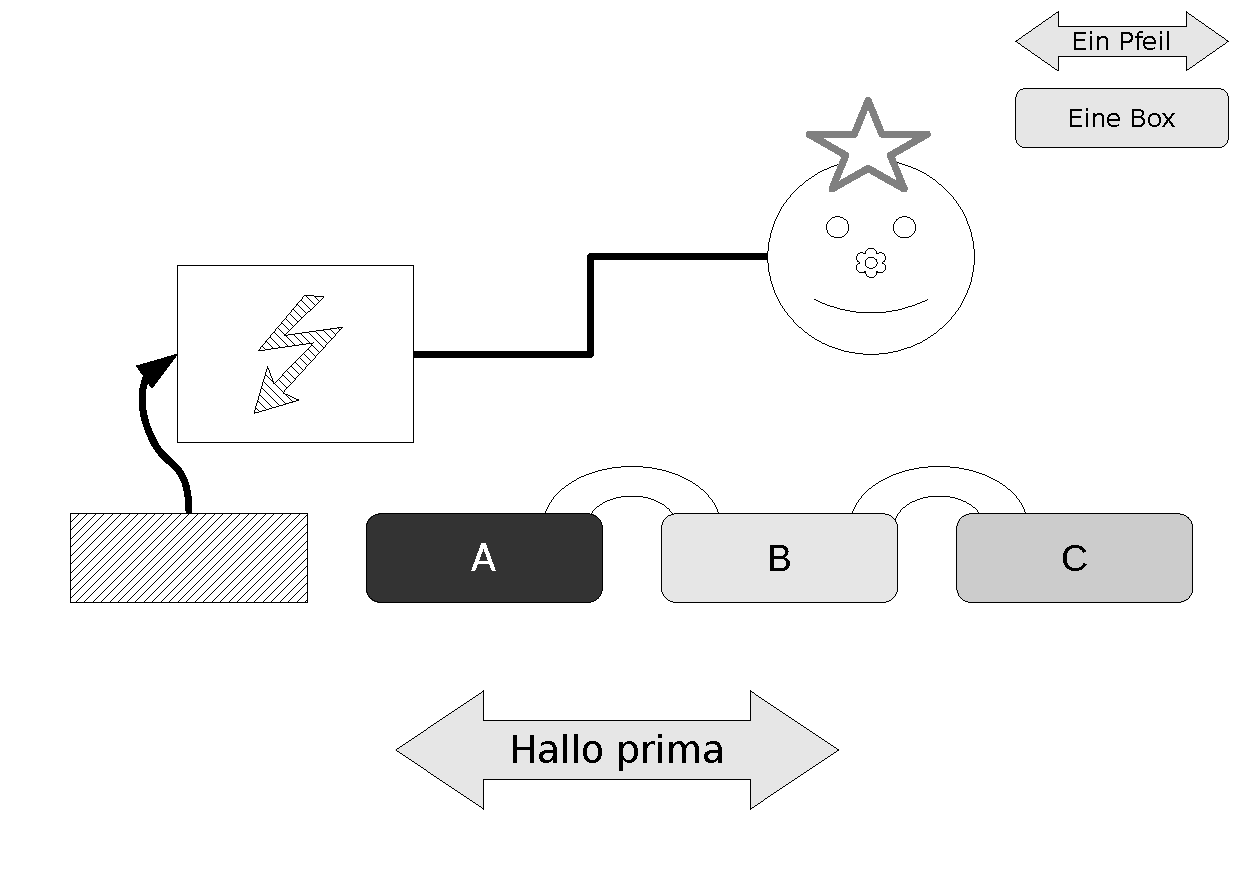
\includegraphics[width=.9\textwidth]{zeichnung.eps}
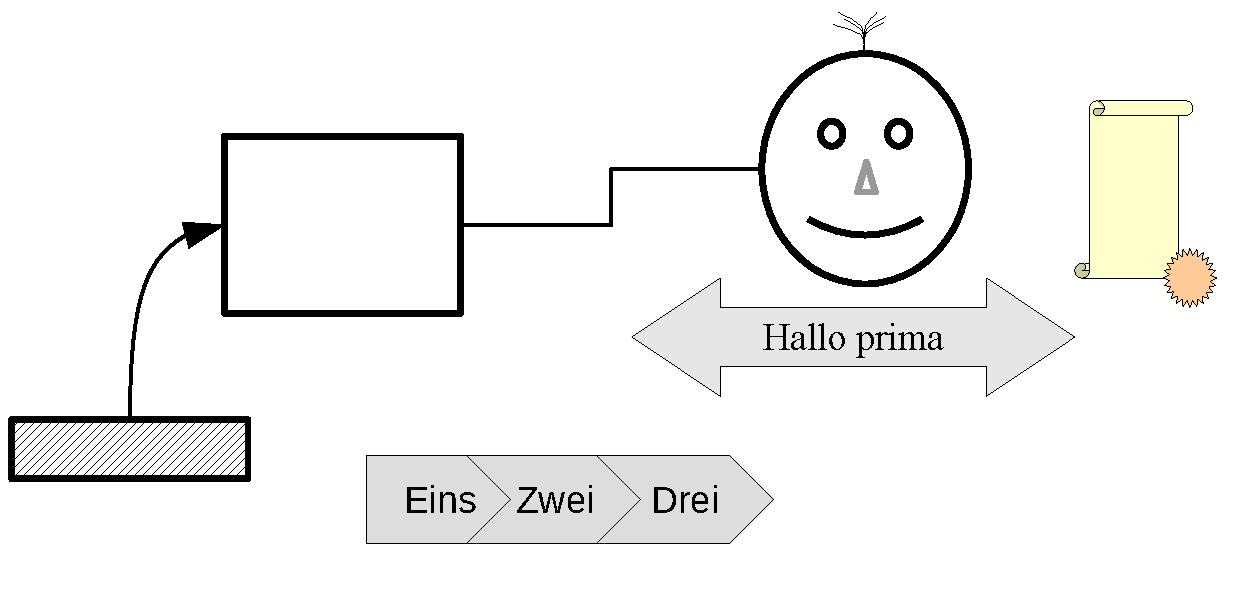
\includegraphics[width=.9\textwidth]{zeichnung.pdf}
\caption{Die tolle Konzeptzeichnung}
\label{fig:tk}
\end{figure}

Auch wenn der Code mal länger wird, wie in Listing~\ref{code:ggtaua}, 
was ja eigentlich in einer Ausarbeitung gar nicht vorkommt, 
dann sollte man den Code als Fließobjekt setzen und 
zusätzlich auch nie so lange Text schreiben wie der hier, der sich 
über mehre Zeilen zieht und einen ganzen Absatz repräsentiert, 
weil viele, und das zu Recht, lange Texte, die auch noch verschachtelt sind,
oder schlimmeres, einfach nicht lesbar finden und man schnell
die Übersicht verliert, was hier passiert ist.
Kurze Sätze sind besser. 

\begin{listing}[ht]
\begin{lstlisting}
def ggt(x, y):
    if x == y or x == 1 or y == 1:
        return min(x,y)
    if x > y:
        x,y = y,x
    # es gilt x < y
    return ggt(x, y-x)
\end{lstlisting}
\caption{Listing ggt -- lang und schlecht}
\label{code:ggtaua}
\end{listing}

Und wenn man dann am Schluss ein PDF~\cite{pdf} macht, dann
sollten darin auch die Fonts gut aussehen. 
Die Fonts sollen beim Vergrößern nicht pixeln (Bitmap-Fonts) sondern
schön skalieren. 
Mit der Zeile 
\begin{verbatim}
  \usepackage{mathptmx}
\end{verbatim}
verwendet man Postscript-Times Schriften statt
\newcommand{\cmr}{\fontfamily{cmr}\fontseries{m}\fontsize{11}{14}\selectfont}
{\cmr Computer Modern Roman}.
Das sieht auf günstigen Druckern ($< 2400$ dpi) besser aus und
pixelt eigentlich auch nie.
Jetzt nochmal eine Online-Quelle wie Wikipedia~\cite{wikipedia} 
und wie man mit Wikipedia zitiert~\cite{wikipedia,wikipediaciting},
auch wenn man dies vermeiden sollte.


\section{Zusammenfassung und Ausblick}

\LaTeX\ ist also sehr nett.
Man kann sich beim Schreiben auf den Inhalt konzentrieren,
man gibt nur die Struktur vor und das Layout wird professionell gesetzt.
Abbildungen, Tabellen und anderes wird als Fließobjekte eingebunden.
Es gibt nichts besseres für Literaturangaben.

Wer will kann noch Farben verwenden, mit \LaTeX\ 
malen\footnote{In \LaTeX\ zu malen ist nur was für Hartgesottene.},
rechnen, \ldots.
Aber dazu gibt es ausreichend Doku,
wie zum Beispiel den Kopka~\cite{kopka}.


% \newpage
% Listen, wenn überhaupt!, bitte ans Ende und nicht an den Anfang
%\listoffigures % Liste der Abbildungen 
%\listoftables % Liste der Tabellen
% wenn es nach mir geht, weglassen

% \newpage % in einer kurzen Ausarbeitung weglassen
% Als letztes noch das Literaturverzeichnis
\bibliographystyle{plainurl} % mit url
\bibliography{ausarb,online}
% dann mit "bibtex ausarb" bibtexen und das Literaturverzeichnis ist da
% Besser wäre es mit bibtopic die Quellen sauber zu trennen, siehe thesis

\end{document}
